\documentclass[UTF8]{ctexart}
\usepackage{geometry, CJKutf8}
\geometry{margin=1.5cm, vmargin={0pt,1cm}}
\setlength{\topmargin}{-1cm}
\setlength{\paperheight}{29.7cm}
\setlength{\textheight}{25.3cm}

% useful packages.
\usepackage{amsfonts}
\usepackage{amsmath}
\usepackage{amssymb}
\usepackage{amsthm}
\usepackage{enumerate}
\usepackage{graphicx}
\usepackage{multicol}
\usepackage{fancyhdr}
\usepackage{layout}
\usepackage{listings}
\usepackage{float, caption}


\lstset{
	basicstyle=\ttfamily, basewidth=0.5em
}

% some common command
\newcommand{\dif}{\mathrm{d}}
\newcommand{\avg}[1]{\left\langle #1 \right\rangle}
\newcommand{\difFrac}[2]{\frac{\dif #1}{\dif #2}}
\newcommand{\pdfFrac}[2]{\frac{\partial #1}{\partial #2}}
\newcommand{\OFL}{\mathrm{OFL}}
\newcommand{\UFL}{\mathrm{UFL}}
\newcommand{\fl}{\mathrm{fl}}
\newcommand{\op}{\odot}
\newcommand{\Eabs}{E_{\mathrm{abs}}}
\newcommand{\Erel}{E_{\mathrm{rel}}}

\begin{document}
	
	\pagestyle{fancy}
	\fancyhead{}
	\lhead{王琰博, 3220105837}
	\chead{数据结构与算法第七次作业}
	\rhead{Nov.29th, 2024}
	
	\section{测试程序的设计思路}
	
	根据评分标准中要求,我们首先对HeapSort.h进行设计。我把实现堆排序分为两步,首先是将序列转化为最大数为根节点,所有子节点比父节点小的形式。为此我设计了调整堆(表现形式为数组)的函数adjustHeap,该函数通过递归的方式调整数组中元素的位置,将二叉树调整为上述最大数为根节点的形式。
	在调整结束之后,即可用Heapsort函数对该堆进行排序。通过循环不断地将此堆中的最大值取出放在数组的末尾,在通过上述adjustHeap函数调整新的堆,即可得到一个升序的序列,排序完成。

	
	\begin{figure}[H] %H为当前位置,!htb为忽略美学标准,htbp为浮动图形
		\centering %图片居中
		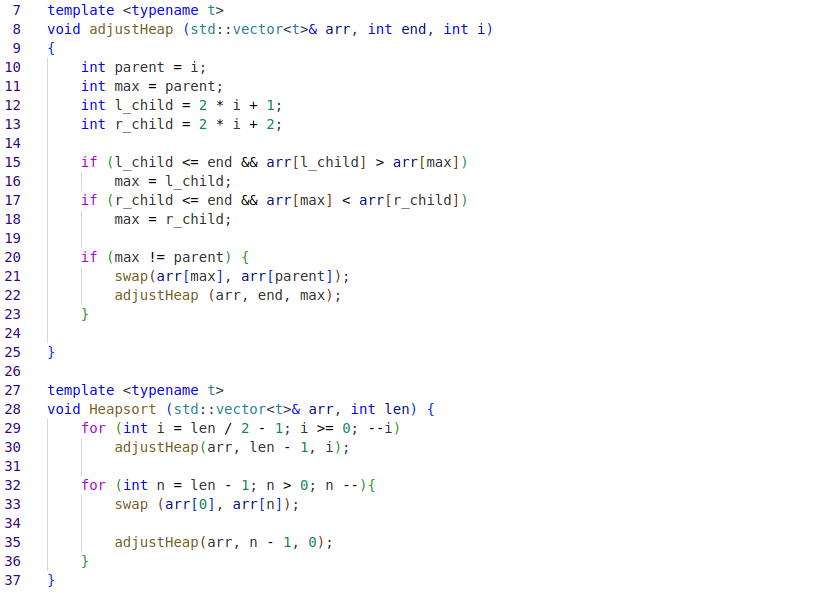
\includegraphics[width=0.7\textwidth]{fig1} %插入图片,[]中设置图片大小,{}中是图片文件名
		\caption{function in HeapSort.h} %最终文档中希望显示的图片标题
	\end{figure}
	
	随后我们设计test.cpp文件中的函数。
	
	关于检测排序正确性的check函数比较简单。因为我们最终生成一个升序序列,所以只循环比较每一组前后元素的大小即可验证最终排序是否为升序序列。若前一个元素更大,则证明排序错误
	
	\begin{figure}[H] %H为当前位置,!htb为忽略美学标准,htbp为浮动图形
		\centering %图片居中
		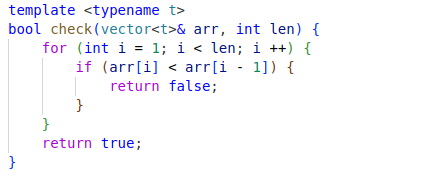
\includegraphics[width=0.7\textwidth]{fig2} %插入图片,[]中设置图片大小,{}中是图片文件名
		\caption{function check} %最终文档中希望显示的图片标题
	\end{figure}
	
	除此之外我设计了一个生成随机序列的函数RandomQ,其中第一个序列vAllIndices是存放随机数值的序列,而第二个序列vAvaibleIndices则是存放索引的序列。通过随机数取模的hash手段来构建一个简单的随机序列,为了尽量保证不碰撞需要设计随机数值大于索引。
	
	
	\begin{figure}[H] %H为当前位置,!htb为忽略美学标准,htbp为浮动图形
		\centering %图片居中
		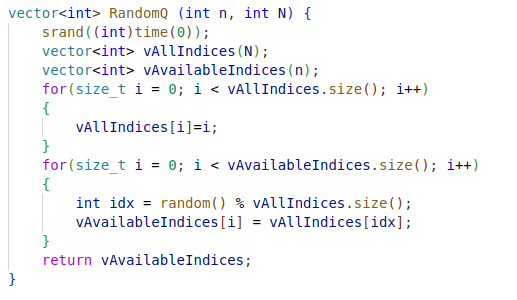
\includegraphics[width=0.7\textwidth]{fig3} %插入图片,[]中设置图片大小,{}中是图片文件名
		\caption{function RandomQ} %最终文档中希望显示的图片标题
	\end{figure}
	
	
	
	最后则是主函数的设计。首先是对变量进行初始化,重复序列随机数值设定为0-1000,随机序列随机数值设定为0-100000000。之后的测试中首先都是生成序列,然后再深度拷贝出另一个序列以分别采用sort\_heap函数和Heapsort函数进行排序。同时利用chrono进行计时。最后根据check函数的判断结果输出测试是否通过。正序逆序序列就用累加累减生成。
	
	\begin{figure}[H] %H为当前位置,!htb为忽略美学标准,htbp为浮动图形
		\centering %图片居中
		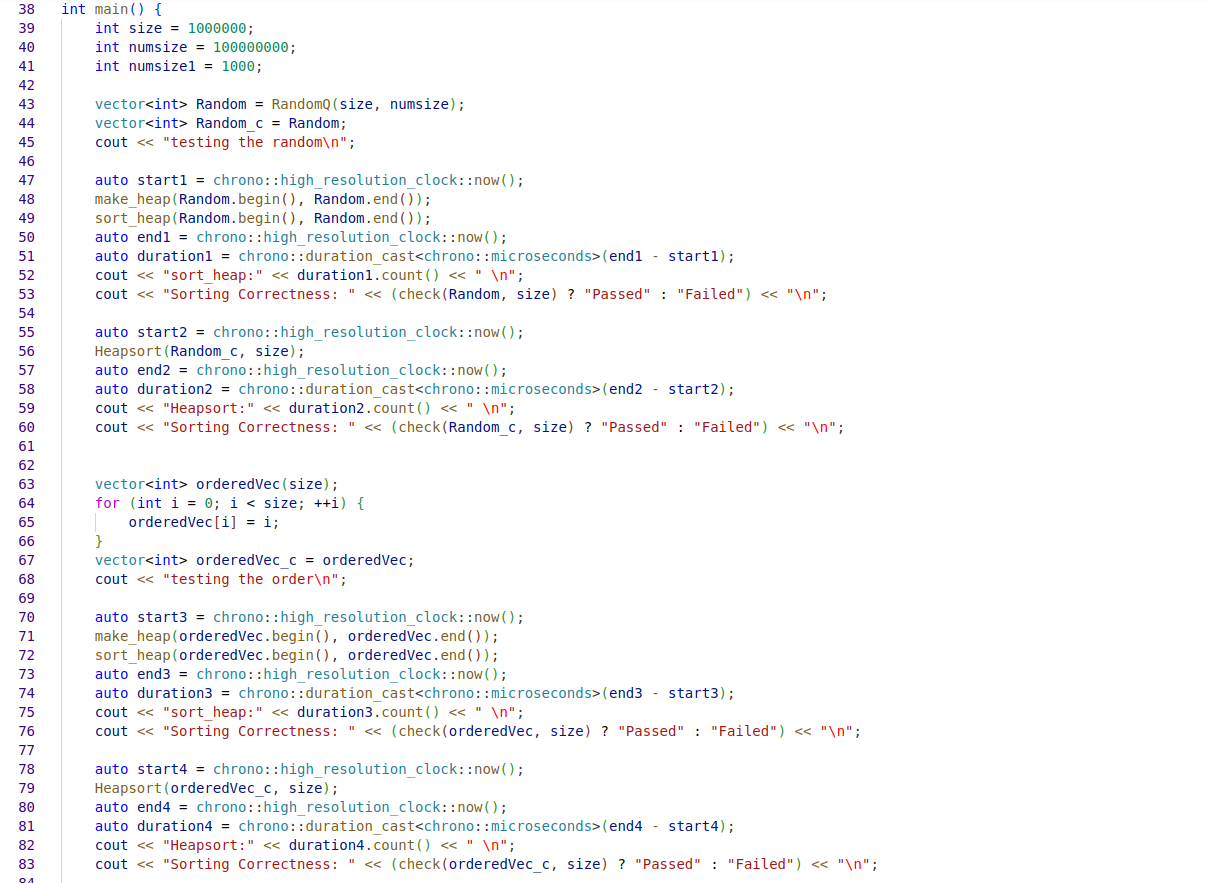
\includegraphics[width=0.7\textwidth]{fig4} %插入图片,[]中设置图片大小,{}中是图片文件名
		\caption{main} %最终文档中希望显示的图片标题
	\end{figure}
	
	\begin{figure}[H] %H为当前位置,!htb为忽略美学标准,htbp为浮动图形
		\centering %图片居中
		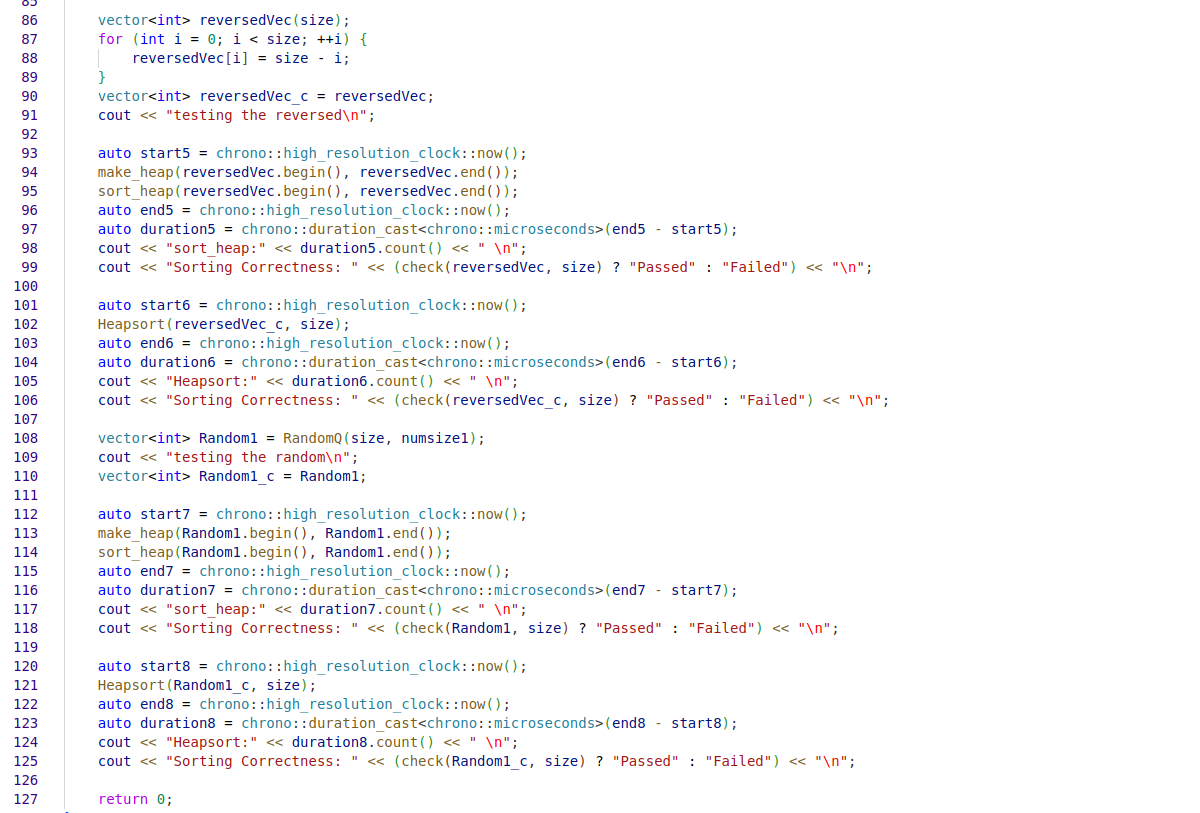
\includegraphics[width=0.7\textwidth]{fig5} %插入图片,[]中设置图片大小,{}中是图片文件名
		\caption{main} %最终文档中希望显示的图片标题
	\end{figure}

	
	\section{测试的结果}
	
	
	输出为: 
	
	\begin{figure}[H] %H为当前位置,!htb为忽略美学标准,htbp为浮动图形
		\centering %图片居中
		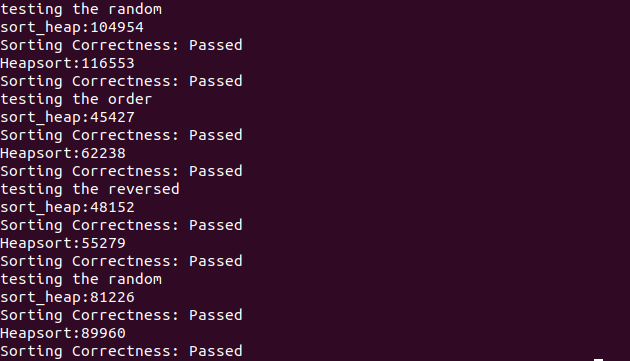
\includegraphics[width=0.7\textwidth]{fig6} %插入图片,[]中设置图片大小,{}中是图片文件名
		\caption{output} %最终文档中希望显示的图片标题
	\end{figure}





	表格为:
	
	\begin{table}[H]
		\centering
		\begin{tabular}{|l|l|l|}
			\hline
			~ & my heapsort time & std::sort\_heap time \\ \hline
			random sequence & 116553 & 104954 \\ \hline
			ordered sequence & 62238 & 45427 \\ \hline
			reverse sequence & 55279 & 48152 \\ \hline
			repetitive sequence & 89960 & 81226 \\ \hline
		\end{tabular}
		\caption{the result}
	\end{table}
	
	\section{bug报告}
	
	一切正常。
	
	%%% Local Variables: 
	%%% mode: latex
	%%% TeX-master: t
	%%% End: 
\end{document}